\section{Finding Bottleneck Flow}
\label{sec:bottleneck}

Again, we turn to the satisfiability equation, but use random variables for the Traffic Factor and Path Length, $TF_i$ and $PL_i$, respectively:
\begin{equation}
	T \geq \frac{ k_{req} \cdot I_S \cdot CF \cdot TF_i}{W} + \frac{P_S \cdot DF \cdot (PL_i-1)}{W}
\end{equation}
where we will call the total delay
\begin{equation}
	D_i = \frac{ k_{req} \cdot I_S \cdot CF \cdot TF_i}{W} + \frac{P_S \cdot DF \cdot (PL_i-1)}{W}
\end{equation}

Now, we want to identify which flow $i$, identified by its origin node, is most likely to be the flow that cannot be satisfied in the allotted timeliness.  To do so, we can simply find the value of $i$ that results in the largest $D_i$.

\begin{figure}
\begin{centering}
    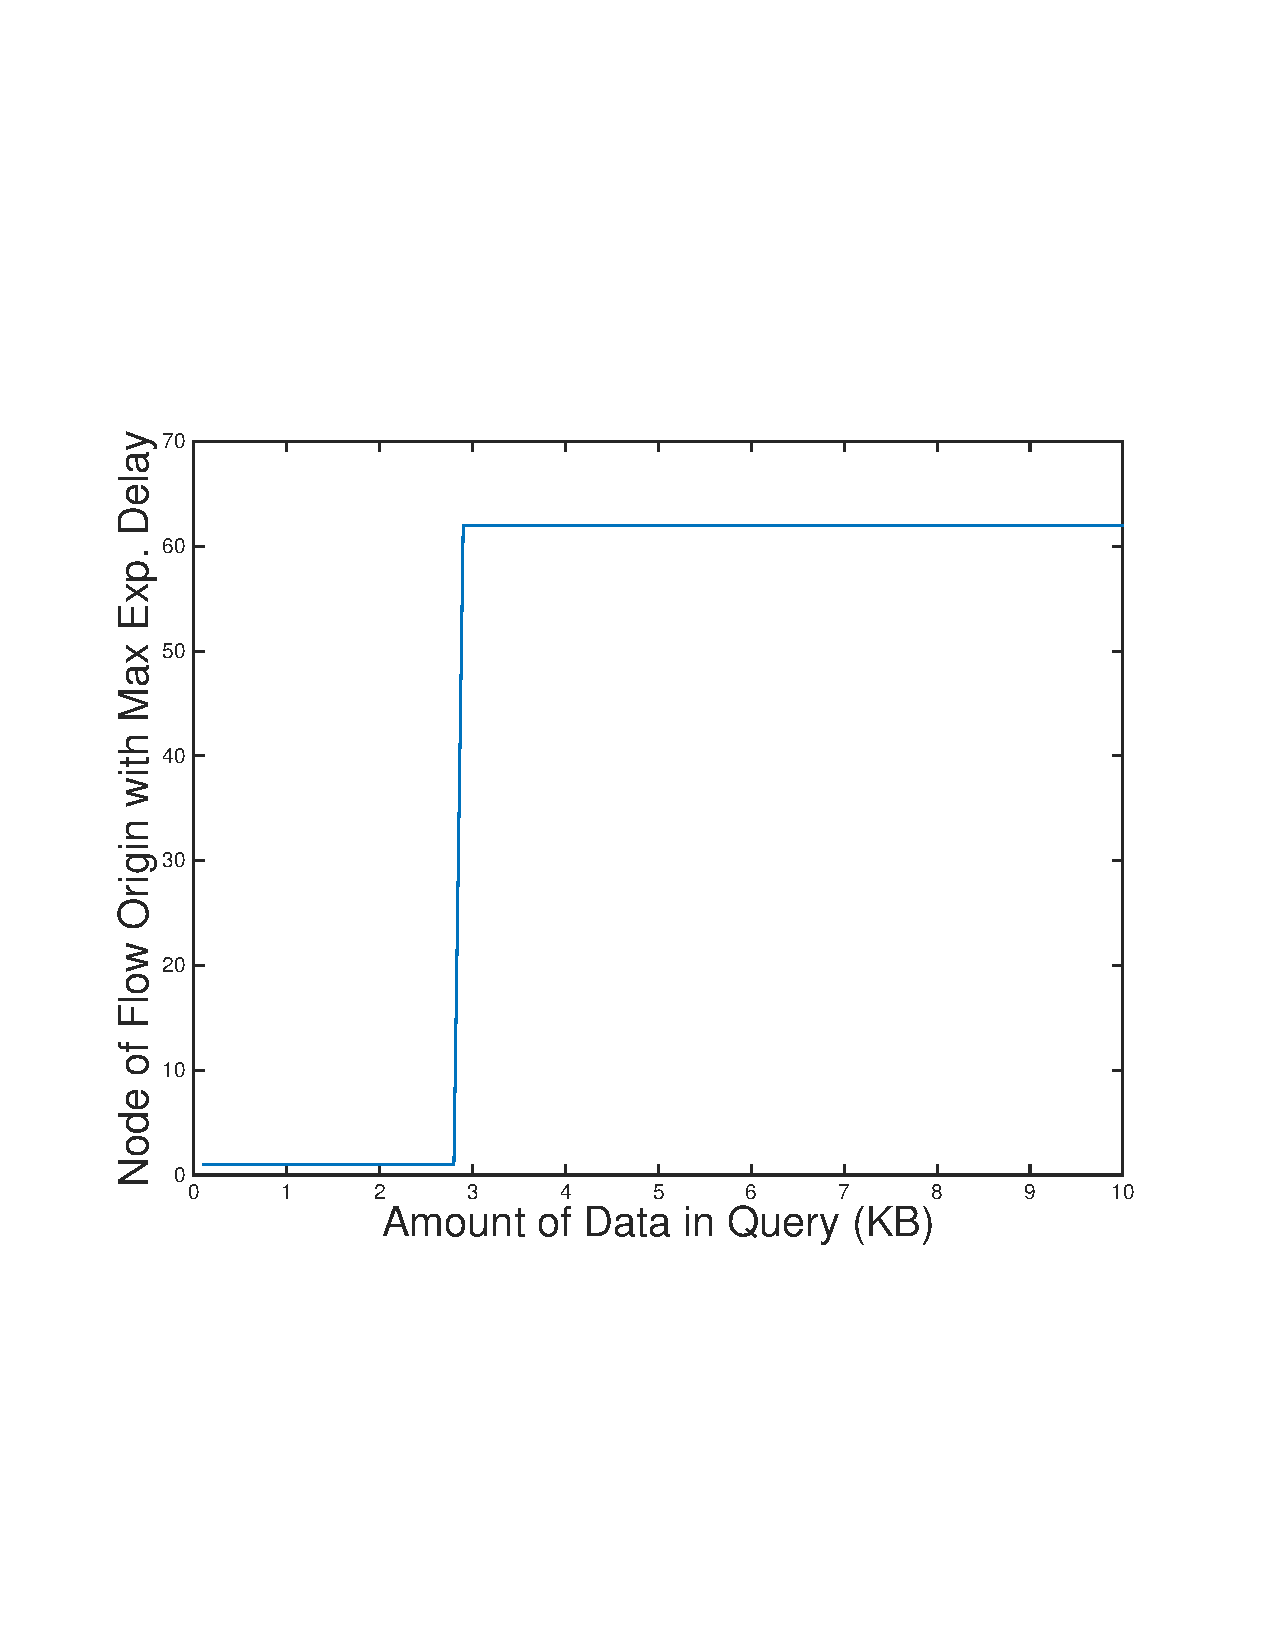
\includegraphics[scale=0.4, clip=true, trim=15mm 65mm 20mm 65mm]{figures/max_i_line_net_125.pdf}
    \caption{The value of $i$ (origin of a flow) that causes the maximum expected delay.}
    \label{fig:max_i_line_net}
\end{centering}
\end{figure}

Using the expected values for $TF_i$ and $PL_i$ from Figures \ref{fig:EV_TF_line_net} and \ref{fig:mean_PL_each_node_line_net}, we find the value of $i$ that maximizes $D_i$ for different data requirements, $B = k_{req}*I_S$.  Figure \ref{fig:max_i_line_net} shows that for low data requirements, the delay of multi-hop paths dominates, causing the ``Bottleneck" flow to be those that originate in node $1$ and have a larger expected path length.  At a point, though, as the amount of data required in the query grows, congestion will be the limiting factor in the network, making the Traffic Factor more important.  Thus, the node near the center of the network which will be likely to experience the highest amount of congestion become the source of flows with the highest delay.  In this case, we have $i = 62$, since the network has $125$ nodes (NOTE: It should probably be 63, but there is an ``off-by-one" error here because the definitions/formulations are not carefully derived to be correct on the boundaries).

